\section{Methods}\label{meth}
%---------------------------------------------------------------------------------------------------
\subsection{Risk Group Duration}\label{meth.group}
\begin{figure}
  \centering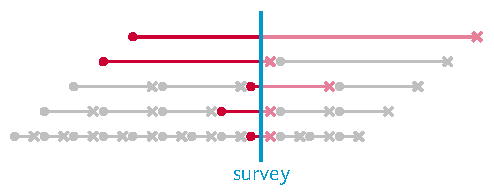
\includegraphics[scale=1]{diag.group}
  \caption{TODO}
  \label{fig:diag.group}
\end{figure}
%---------------------------------------------------------------------------------------------------
\subsection{Sexual Partnership Duration}\label{meth.partners}
Sexual partnerships are often quantified from cross-sectional survey data.
Respondents are typically asked to report
their numbers of unique partners ($x$) during a standardized recall period ($\omega$) --- \eg
\shortquote{How many different people have you had sex with during the past year?}
Such data can then be used to define
a rate of partnership change ($Q$) and/or a number of currrent partnerships ($K$).
\par
If partnership duration ($\delta$) is long and the recall period is short
--- \eg $\omega \approx 0$ for
\shortquote{Are you currently in a long-term sexual partnership?} ---
the reported partnerships mostly reflect \emph{ongoing} partnerships,
and thus $x \approx K$.
If partnership duration is short and the recall period is long
--- \eg $\delta \approx 0$ for
\shortquote{How many one-off sexual partners have you had during the past year?} ---
the reported partnerships mostly reflect \emph{complete} partnerships,
and thus $x/\omega \approx Q$.
However, if partnership duration and recall period are similar in length,
the reported partnerships reflect a mixture of tail-ends, complete, and ongoing partnerships,
and thus $x$ overestimates $K$, but $x/\omega$ also overestimates $Q$.
\par
One solution to this problem would be to ask respondents about
\emph{new} partnerships ($x'$) during the recall period,
which can give an unbiased estimate of the change rate as: $Q = x'/\omega$.
However, for surveys do not include these data,
an unbiased estimator for $Q$ and $K$ that uses
\emph{all} reported partnerships in the recall period ($x$) would be useful.
\par
We take the partnership duration to be fixed and known.
We start with a similar assumption as in \sref{meth.group}:
that survey timing is effectively random with respect to partnership duration.
Then, if either end of the recall period would capture an ongoing partnership,
the intersection point would be, on average, at the partnership mid-point.
Thus, the recall period is effectively extended
by half the partnership duration $\delta/2$ on each end, and $\delta$ overall,
as illustrated in Figure~\ref{fig:diag.partners}.
As such, we can define $Q$ and $K$ as:
\begin{alignat}{1}
  Q &= \frac{x}{\omega + \delta}\\
  K &= \frac{x \delta}{\omega + \delta} = Q \delta
\end{alignat}
\par
As an example, Figure~\ref{fig:diag.partners} also illustrates
a recall period of $\omega = 1$ year,
for which $x = 9$ partnerships are reported,
having durations of $\delta = 9$ months.
Thus, we can compute
$Q = 9/(1+0.75) = 5.14$ partnerships per year and
$K = 5.14(0.75) = 3.86$ current partners;
these ars slight underestimates of the true values $Q = 5.33, K = 4$,
due to randomness in the exact ``location'' of the recall period.
\begin{figure}
  \centering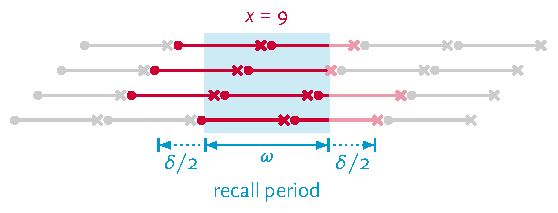
\includegraphics[scale=1]{diag.partners}
  \caption{TODO}
  \label{fig:diag.partners}
\end{figure}
